\documentclass[10.5pt]{ctexart}
\usepackage{graphicx}
\usepackage{indentfirst}
\usepackage[a4paper, inner=1.5cm, outer=3cm, top=2cm, bottom=3cm, bindingoffset=1cm]{geometry}
\usepackage{epstopdf}
\usepackage{array}
\usepackage{fontspec}
\usepackage{gensymb}
\usepackage[lofdepth,lotdepth]{subfig}
\setlength{\extrarowheight}{4pt}
\begin{document}
\title{\textbf{\fontsize{15.75pt}{\baselineskip}{恒温槽实验报告}}} % 15.75pt is 3 号 in chinese
\author{\fontsize{12pt}{\baselineskip}{数33 赵丰 2013012178 \quad 助教:韩强}}
\date{\fontsize{12pt}{\baselineskip}{9 19,2016}}
\maketitle
\section{\textbf{\fontsize{12pt}{\baselineskip}{引言}}}
本次实验用实验室的仪器依照原理图自行搭建一恒温槽装置,实现使大烧杯中的水温维持恒定的功能,计算表明一般状态下我搭建的恒温槽装置可维持温度在30$\pm0.05$\degree C。若适当调小变压器的输入电压增大磁力搅拌器的速率,可进一步提高控温的精度。通过本实验了解控温与测温的原理,并学会用计算机采集数据。
\section{\textbf{\fontsize{12pt}{\baselineskip}{实验操作}}}
\subsection{\textbf{\fontsize{12pt}{\baselineskip}{实验药品、仪器型号及测试装置示意图}}}
本次实验用到的主要仪器如下图所示:
\begin{figure}[!ht]
\centering
\caption{恒温槽实验主要装置照片}
\includegraphics[width=400pt]{Equipment.png}
\end{figure}


本次实验的仪器主要可分为控温和测温两大模块,其中测温采用了惠斯通电桥法将热敏电阻的电压值转化为电桥两端的电压差值,经无纸记录仪线性
放大后输入到计算机中对数据进行实时处理。控温的原理图如下:
\begin{figure}[!ht]
\centering
\caption{控温原理示意图}
\includegraphics[width=400pt]{PrincipleFigure01.pdf}
\end{figure}


该控温装置为一闭环控制系统,实验中发现该系统的灵敏度不够高,这可能是热得快加热功率过大以及恒温槽温度分布不均所致。
\subsection{\textbf{\fontsize{12pt}{\baselineskip}{实验条件}}}
本次实验在室温,一个大气压的条件下进行。
\subsection{\textbf{\fontsize{12pt}{\baselineskip}{实验操作步骤及方法要点}}}
\begin{enumerate}
\item 在搭好的实验装置基础上接通电源。
\item 搅拌置4档,加热电压即变压器原边电压控制在180V,当节点温度计的示数接近30\degree C 时将加热电压降至100V。
\item 恒温槽升温时使用计算机中的M400接口软件检测输入电压的变化。会发现其一直上升,这表示温度的升高,二者近似为线性关系。
\item 当温度升至30\degree C 且基本维持稳定后,可调节M400纵轴电压的比例,观察到温度随时间变化的曲线(T-t figure)。
\label{MYTtFigure}
\item 在不改变搅拌装置位置的情况下调换热得快、控温传感器和测温传感器的相对位置,共3次,比较4种布局下的 T-t figure。
\item 在某种布局下固定搅拌速度为4档不变,改变加热电压分别为80V和130V,比较恒温效果。
\item 在相同的布局下固定加热电压为100V不变,改变搅拌速度分别为3档和5档,比较恒温效果。
\item 停止加热、待恒温槽自然冷却降温,记仪录节点温度计温度与无纸记录仪转换得到的电压。
\end{enumerate}
\section{\textbf{\fontsize{12pt}{\baselineskip}{结果与讨论}}}
\subsection{\textbf{\fontsize{12pt}{\baselineskip}{原始实验数据}}}
在 (\ref{MYTtFigure}) 中利用无纸记录仪采集到的数据对4种布局分别作图如下:
\newpage
\begin{figure}[h]
  \centering
  \subfloat[][布局1]{
  \includegraphics[width=0.4\textwidth]{ConstTemperature/Figure1.pdf}}
  \subfloat[][布局2]{
  \includegraphics[width=0.4\textwidth]{ConstTemperature/Figure02.eps}}
  \qquad
  \subfloat[][布局3]{
  \includegraphics[width=0.4\textwidth]{ConstTemperature/Figure03.eps}}
  \subfloat[][布局4]{
  \includegraphics[width=0.4\textwidth]{ConstTemperature/Figure04.eps}}
  \caption{不同布局下的T-t figure}
\end{figure}


对于(6),(7),T-t figure 如下图所示:
\begin{figure}[!ht]
\centering
\caption{改变加热电压和搅拌速率下的T-t figure}
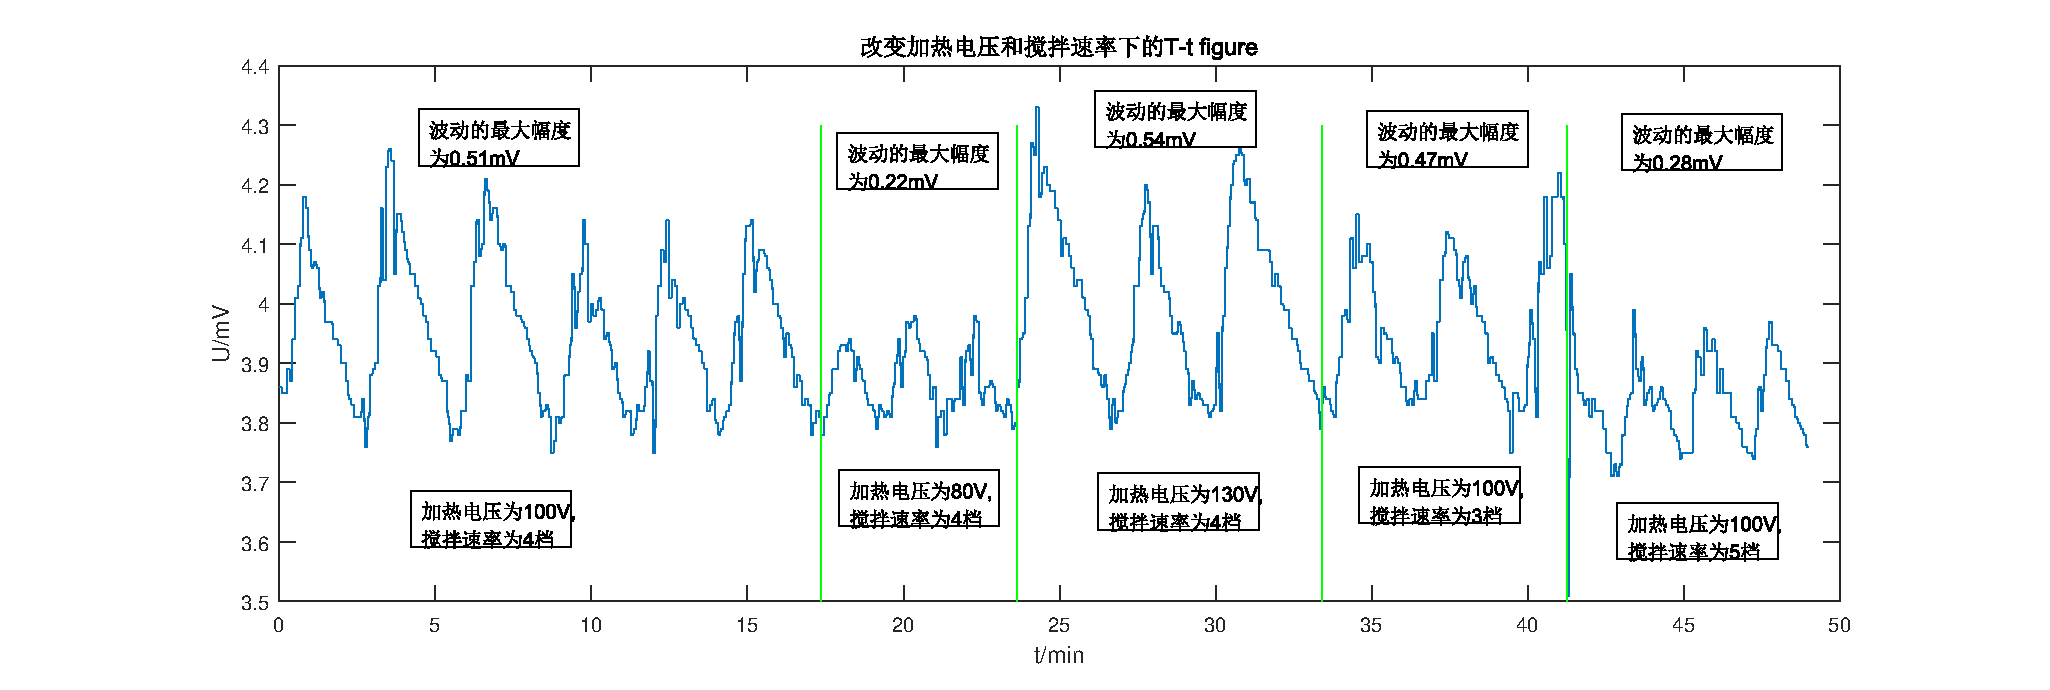
\includegraphics[width=400pt]{ConstTemperature/Figure5.eps}
\end{figure}


对于(8),无纸记录仪电压随温度变化关系如下图所示:
\begin{figure}[!ht]
\centering
\caption{改变加热电压和搅拌速率下的T-t figure \label{fig:UT}}
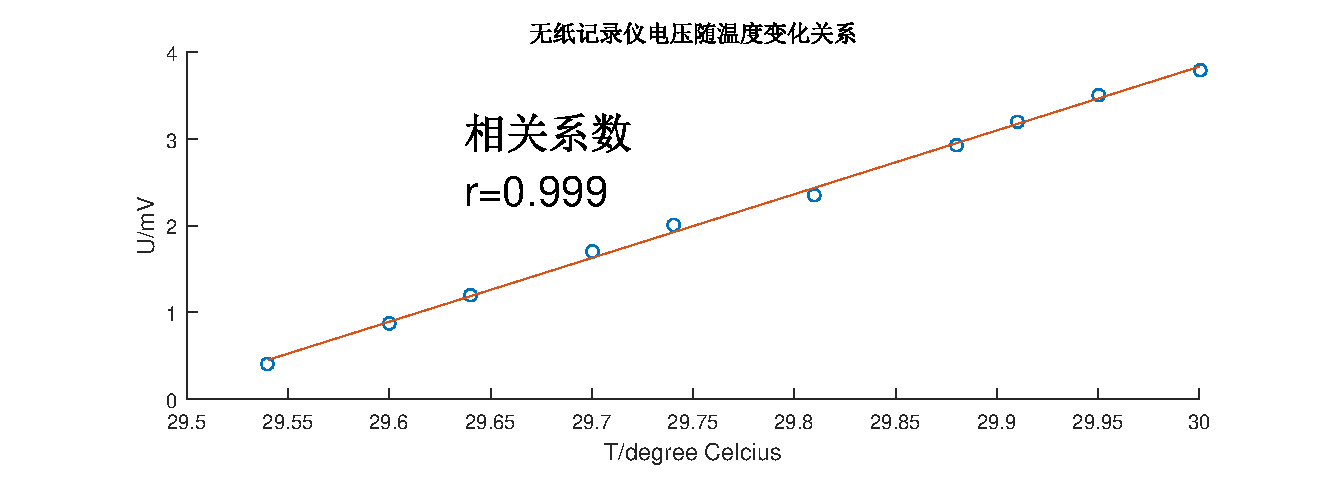
\includegraphics[width=400pt]{ConstTemperature/Figure6.eps}
\end{figure}
\newpage
\subsection{\textbf{\fontsize{12pt}{\baselineskip}{计算的数据、结果}}}

用最小二乘法对 Figure(\ref{fig:UT})中的点进行拟合,进一步可推算出在加热电压为130V,搅拌速率为4档时的平衡温度为30.005 \degree C
及其上限值为30.020\degree C,下限值为29.990 \degree C。从而推出在这种情形下温度的上下波动范围可控制在$\pm0.015$\degree C内。
\subsection{\textbf{\fontsize{12pt}{\baselineskip}{讨论分析}}}
本次实验利用计算机实时处理无纸记录仪采集的大量数据,并且用U-t图的方法呈现给用户,非常直观。

本次实验的改进之处是可以考虑测温的热敏电阻与控温的传感器用一个器件,去掉不必要的水银温度计,以及对无纸记录仪的线性放大部分对实验操作
者提供更充分的说明。

\section{\textbf{\fontsize{12pt}{\baselineskip}{结论}}}

通过本次实验,我们得出如下结论:
\begin{enumerate}
\item 反馈式温度控制装置如设置合理控温精度可达$\pm0.015$\degree C。
\item 一般而言,恒温槽内温度分布有微小的差异,增大搅拌速度可减小这种差异。
\item 反馈式温度控制装置有一定的滞后效应,如减小热得快加热功率可减弱滞后效应带来的控温误差。
\end{enumerate}

\section{\textbf{\fontsize{12pt}{\baselineskip}{参考文献}}}
\begin{thebibliography}{}
\bibitem{Bib1}物理化学实验 \quad 化学工业出版社
\end{thebibliography}
\end{document}